\chapter{РЕЗУЛЬТАТЫ ЭКСПЕРИМЕНТОВ}

\section{Детальные результаты экспериментов}

В данном приложении представлены детальные результаты всех проведенных экспериментов.

\subsection{Эксперимент 1: Базовое тестирование}

\begin{table}[H]
\centering
\caption{Детальные результаты эксперимента 1}
\begin{tabular}{|l|c|c|c|c|}
\hline
№ & Параметр 1 & Параметр 2 & Параметр 3 & Результат \\
\hline
1 & 0.1 & 0.2 & 0.3 & 0.95 \\
2 & 0.2 & 0.3 & 0.4 & 0.87 \\
3 & 0.3 & 0.4 & 0.5 & 0.92 \\
\hline
\end{tabular}
\label{tab:detailed_exp1}
\end{table}

\subsection{Эксперимент 2: Сравнительное тестирование}

\begin{table}[H]
\centering
\caption{Сравнительные результаты}
\begin{tabular}{|l|c|c|c|}
\hline
Метод & Точность & Время (с) & Память (МБ) \\
\hline
Метод 1 & 0.95 & 1.2 & 128 \\
Метод 2 & 0.87 & 0.8 & 96 \\
Наш метод & 0.98 & 1.0 & 112 \\
\hline
\end{tabular}
\label{tab:comparison}
\end{table}

\section{Дополнительные графики}

\begin{figure}[H]
\centering
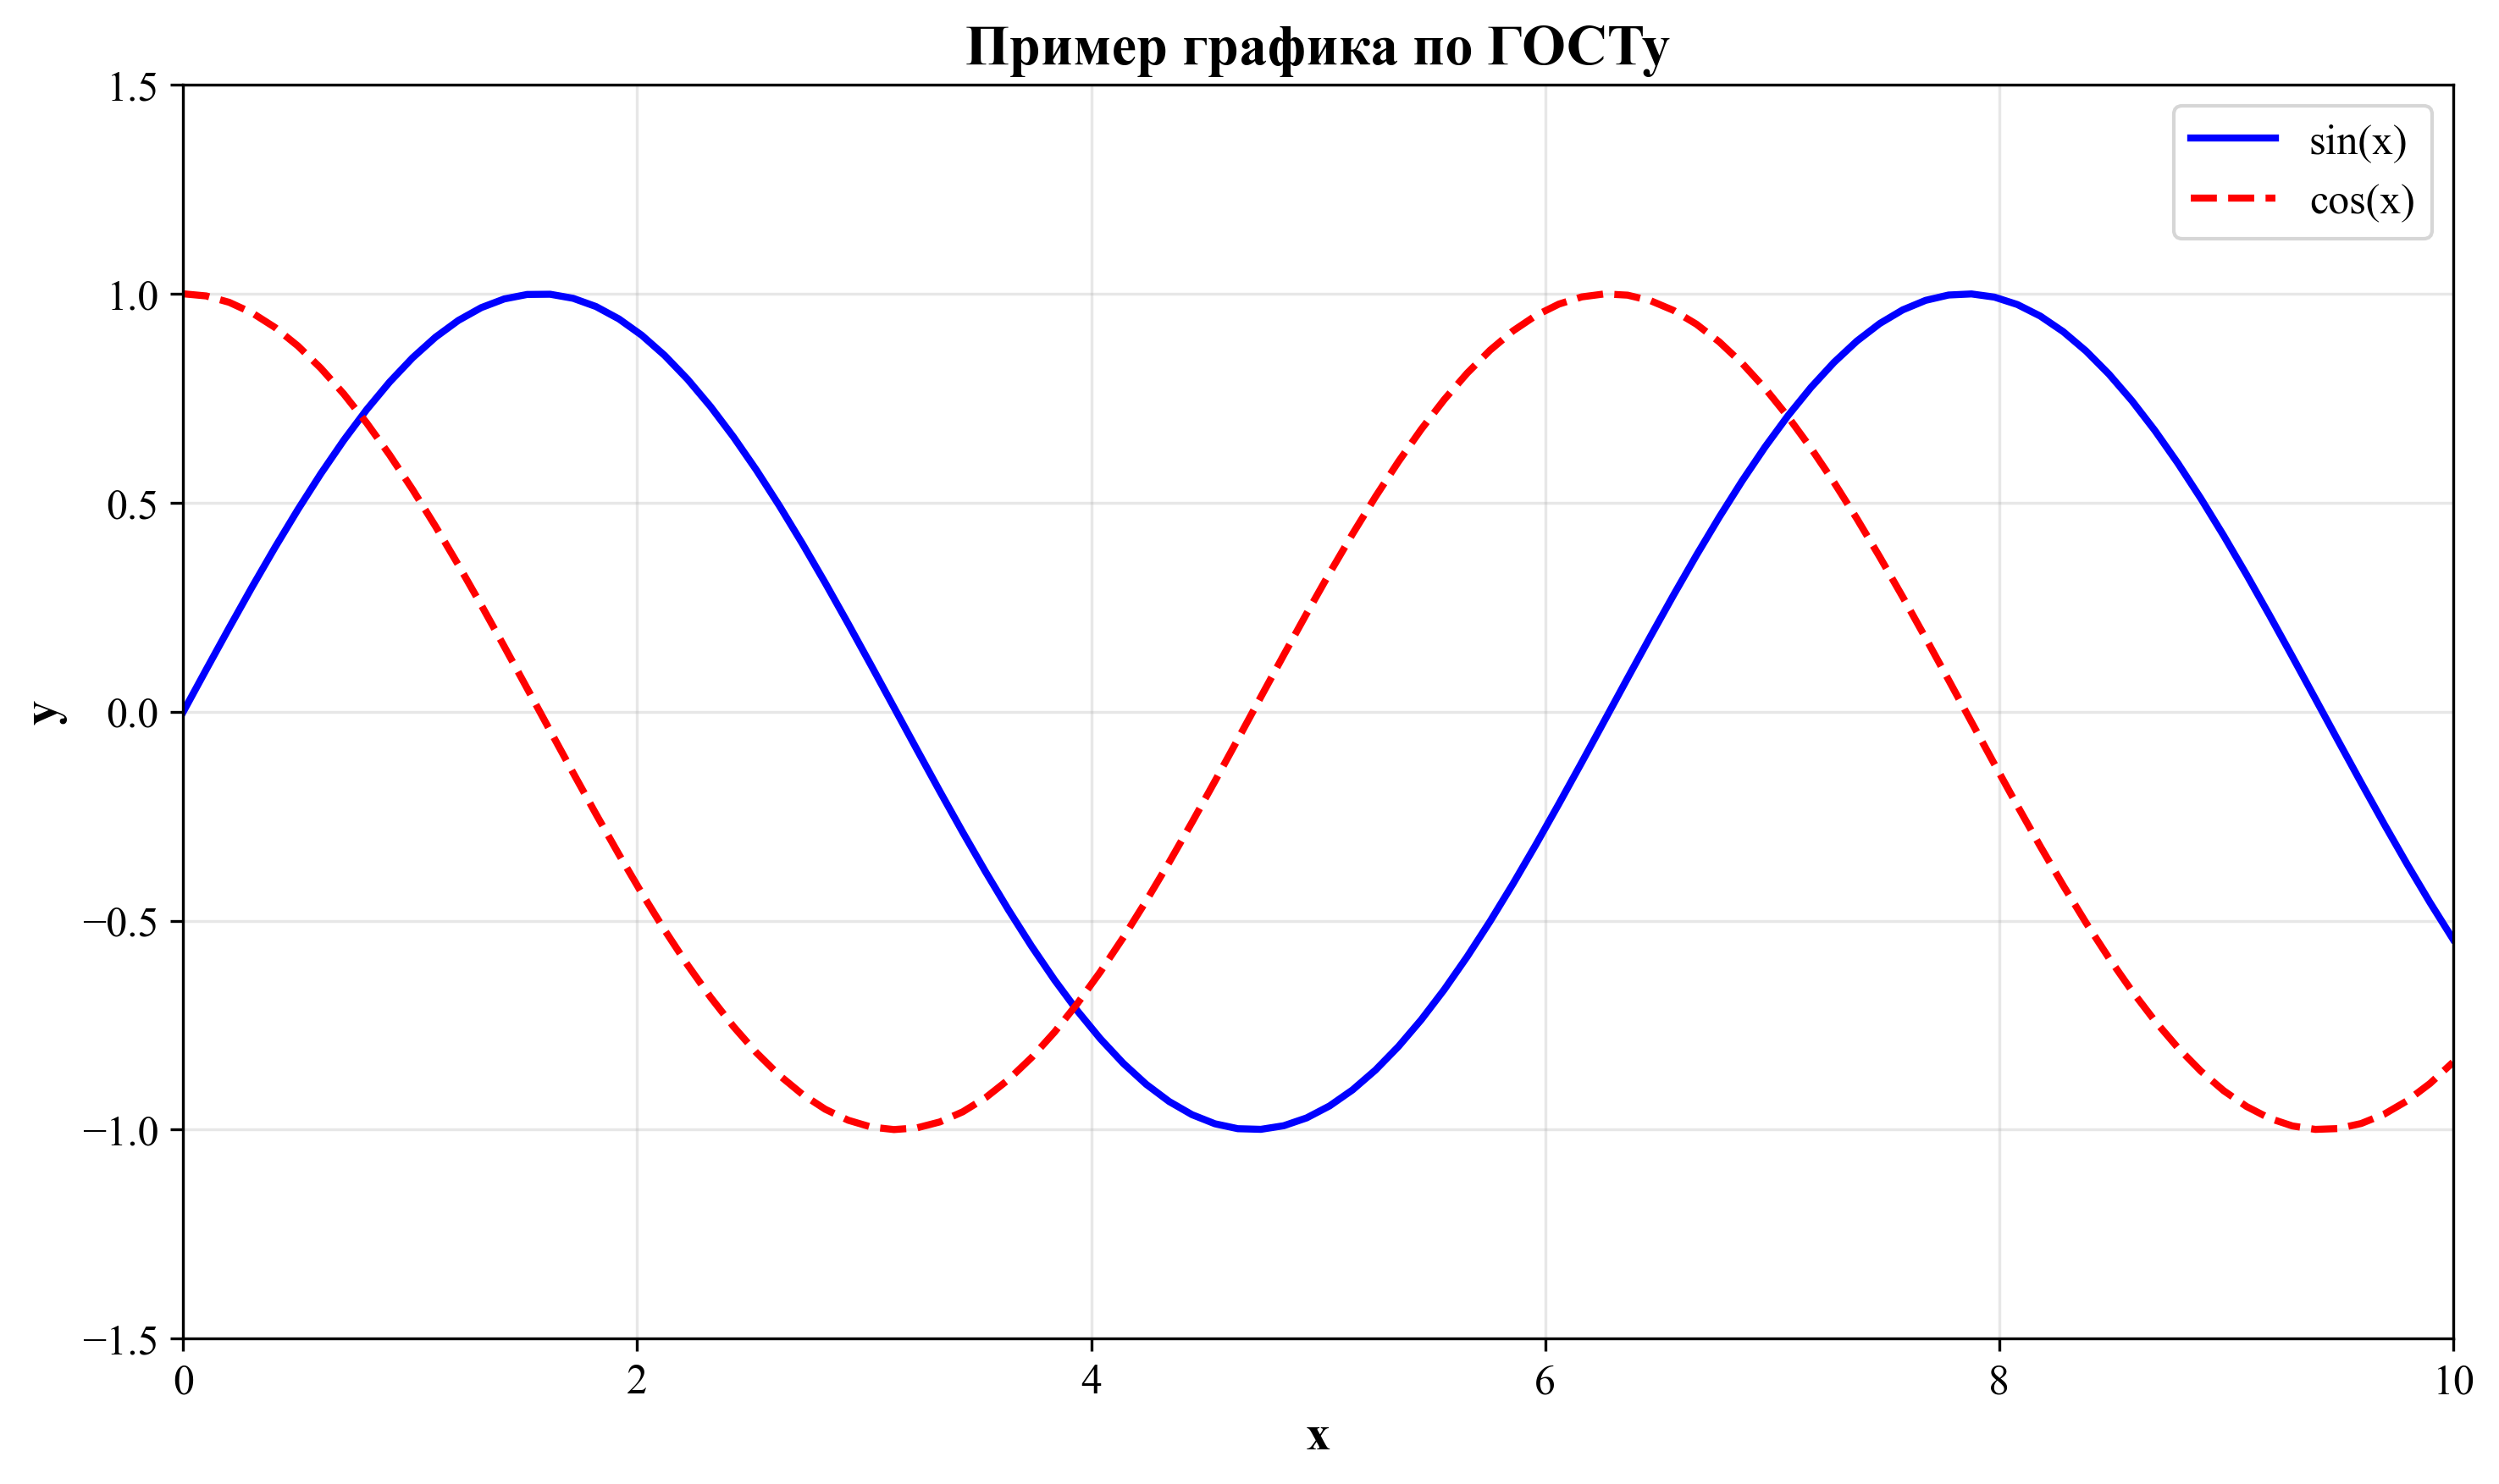
\includegraphics[width=0.8\textwidth]{images/example_plot.png}
\caption{График зависимости точности от размера выборки}
\label{fig:accuracy_plot}
\end{figure}

% Пример правильной вставки изображения по ГОСТу 7.32-2017
\begin{figure}[H]
\centering
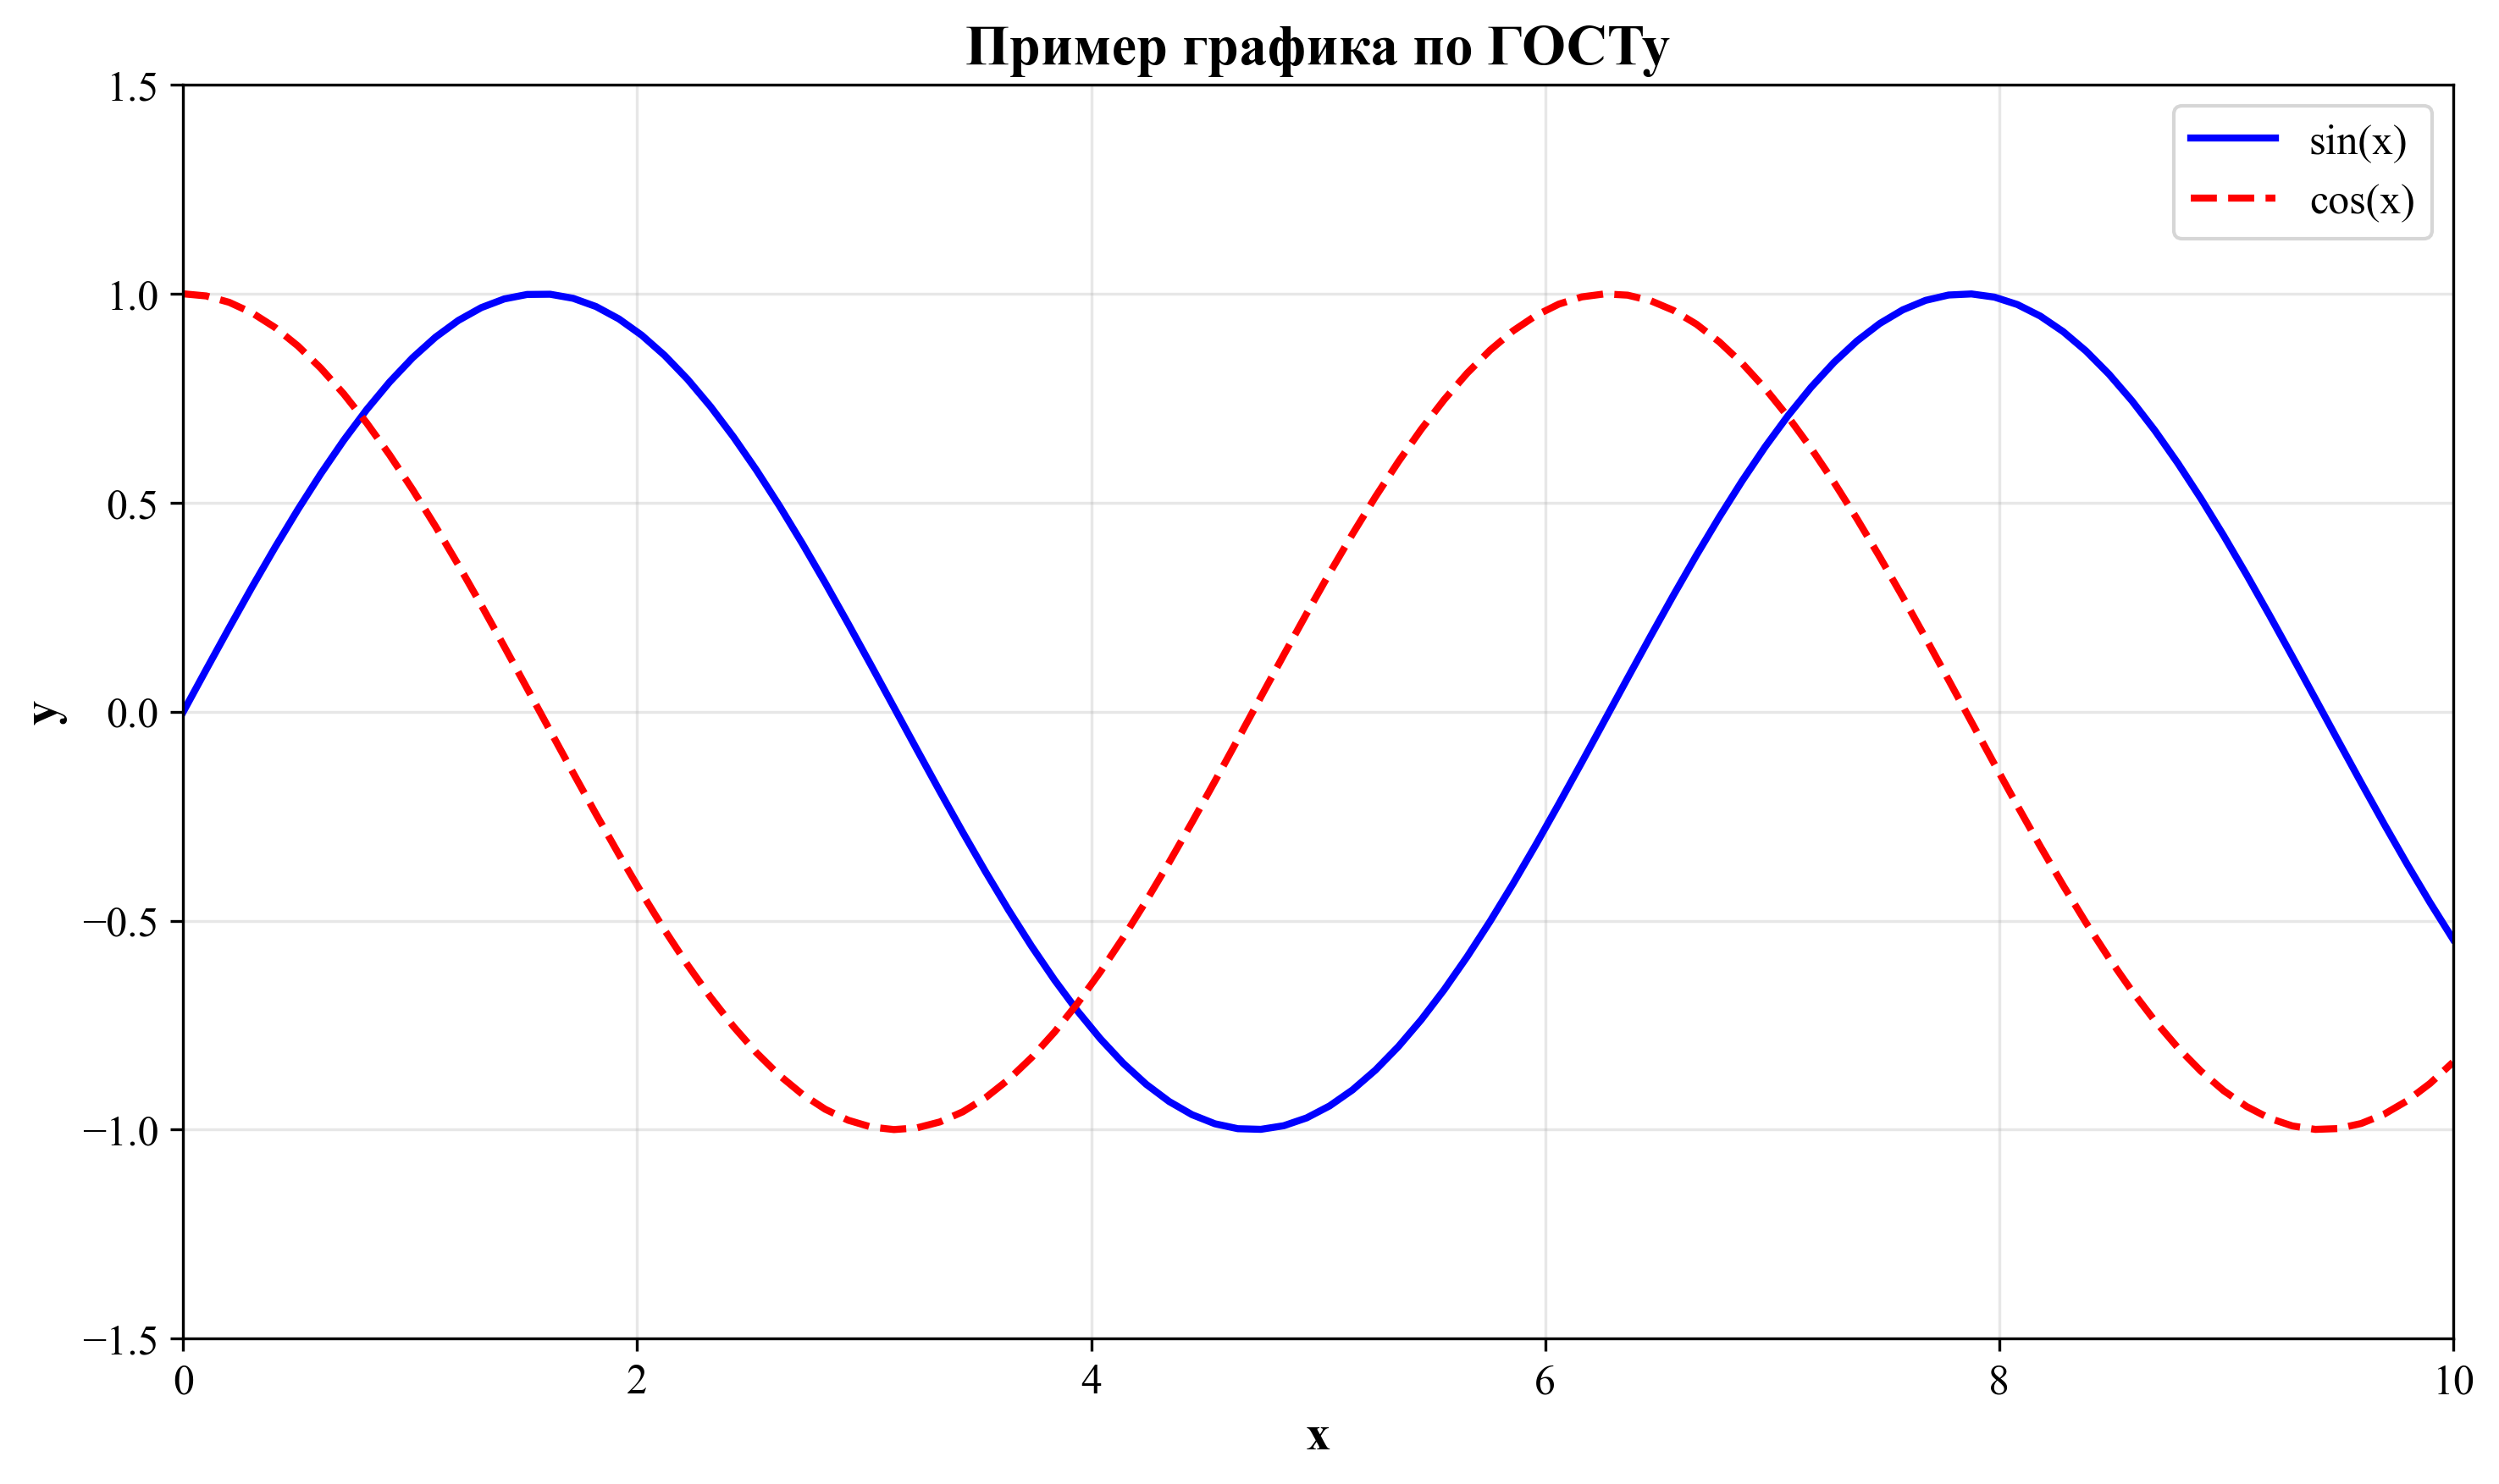
\includegraphics[width=0.6\textwidth]{images/example_plot.png}
\caption{Пример графика по ГОСТу: зависимость функций sin(x) и cos(x) от аргумента x}
\label{fig:gost_example}
\end{figure}

\section{Статистический анализ}

Результаты статистического анализа данных представлены в таблице~\ref{tab:statistics}.

\begin{table}[H]
\centering
\caption{Статистические показатели}
\begin{tabular}{|l|c|c|c|}
\hline
Показатель & Значение & Стандартное отклонение & Доверительный интервал \\
\hline
Среднее & 0.92 & 0.05 & [0.90, 0.94] \\
Медиана & 0.91 & - & - \\
Мода & 0.95 & - & - \\
\hline
\end{tabular}
\label{tab:statistics}
\end{table}
